\documentclass[conference]{IEEEtran}
\IEEEoverridecommandlockouts
% The preceding line is only needed to identify funding in the first footnote. If that is unneeded, please comment it out.
%\usepackage{cite}
\usepackage{amsmath,amssymb,amsfonts}
\usepackage{algorithmic}
\usepackage{graphicx}
\usepackage{textcomp}
\usepackage{xcolor}

\usepackage{pdflscape}

\usepackage[utf8]{inputenc}
\usepackage{fancyhdr}
\usepackage{lastpage}

% Please add the following required packages to your document preamble:
\usepackage{multirow}
\usepackage[numbers]{natbib}

\usepackage{listings}
\usepackage{enumitem}
\usepackage{hyperref}
\usepackage{amsmath}

\hypersetup{
    colorlinks=true,
    linkcolor=black,
    filecolor=magenta,      
	urlcolor=cyan
}

\usepackage{listings}
\usepackage{color}

\definecolor{dkgreen}{rgb}{0,0.6,0}
\definecolor{gray}{rgb}{0.5,0.5,0.5}

\definecolor{mauve}{rgb}{0.58,0,0.82}

\lstset{frame=single,
  language=C++,
  showstringspaces=false,
  columns=flexible,
  basicstyle={\small\ttfamily},
  numbers = none,
  numberstyle=\tiny\color{gray},
  keywordstyle=\color{blue},
  commentstyle=\color{dkgreen},
  stringstyle=\color{mauve},
  breaklines=true,
  breakatwhitespace=true,
  tabsize=2
}

\def\BibTeX{{\rm B\kern-.05em{\sc i\kern-.025em b}\kern-.08em
T\kern-.1667em\lower.7ex\hbox{E}\kern-.125emX}}

\fancypagestyle{fancylandscape}{
\fancyhf{} %Clears the header/footer
\fancyfoot{% Footer
\makebox[\textwidth][r]{% Right
  \rlap{\hspace{.75cm}% Push out of margin by \footskip
    \smash{% Remove vertical height
      \raisebox{4.87in}{% Raise vertically
        \rotatebox{90}{Page \thepage\ of \pageref{LastPage}}}}}}}% Rotate counter-clockwise
\renewcommand{\headrulewidth}{0pt}% No header rule
\renewcommand{\footrulewidth}{0pt}% No footer rule
}

\pagestyle{fancyplain}
\fancyhf{}
\fancyfoot[c]{Page \thepage\ of \pageref{LastPage}}
\renewcommand{\headrulewidth}{0pt}

\begin{document}

	\title{Socket Programming and Concurrency}

	\author{\IEEEauthorblockN{1\textsuperscript{st} Given Edward Patch}
	\IEEEauthorblockA{\textit{Software Engineer Student (of BSc Year 3)} \\
    \textit{Socket Programming and Concurrency}\\
    \textit{University of Wales Trinity St. Davids (of Tim Bashford)}\\
    Swansea, Wales \\
    Student ID: 1801492}}

     \maketitle
    
    \thispagestyle{plain}
    \pagestyle{plain}
    
    %\tableofcontents
	  %\vspace{.5cm}
    %\newpage
    \begin{abstract}
    
    \end{abstract}

    \begin{IEEEkeywords}
        
    \end{IEEEkeywords}

    \section{Introduction}
      This article illustrates interoperability within network protocols and the best way of implementing the method. Network protocols, including Transmission Control Protocol (TCP) and User Datagram Protocol (UDP), explain how they support the networking procedures and ensure data delivery. The synchronisation of the mentioned network protocols gives how I/O dispatch models perform. A problem of a three-way handshake, also known as `Two Generals' and the impacts of Maximum Transmission Unit (MTU) size on data transmission. The article also includes an implementation of a networked Rock, Paper and Scizzors Android Application game that allows a max lobby of two users.

    \section{Network Protocols}
      A network protocol is a set of rules of how a network should handle how network packets (transmission of data) are transmitted and received between network nodes. Usually, the standard template of network protocols comes from an adaptation of the Open Systems Interconnection (OSI) model. Refer to section~\ref{sec:networkModel}, page~\pageref{sec:networkModel}. Designation of the TCP and UDP network protocols fit within the Internet of Things (IoT) category and provides a model that works well with the Internet standard. TCP relies on a connection type protocol, whereas UDP focuses on a connectionless protocol.

      After some observation from the Journal Article, `Experimental Performance Comparison between TCP vs UDP tunnel using OpenVPN' by Irfaan Coonjah~\cite{coonjah_experimental_2015}, the study carried out trials the performance between TCP and UDP using a Virtual Private Network (VPN) tunnel. The VPN platform the the author(s) chose was OpenVPN. Figure~\ref{fig:tcpudp-expset} displays a diagram of the experiment provided by the author~\cite{coonjah_experimental_2015}:-

      \begin{figure}[h]
        \centering
        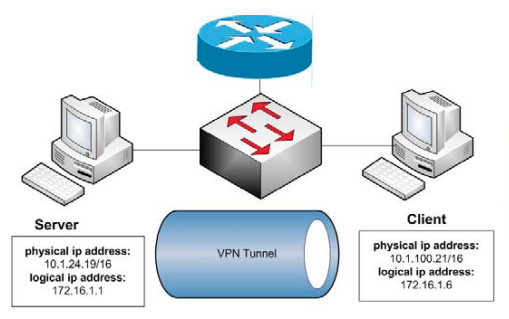
\includegraphics[width=\columnwidth]{Figures/TCPUDP-EXPSET.png}
        \caption{TCP vs UDP Tunnel Experiment Setup~\cite{coonjah_experimental_2015}}
        \label{fig:tcpudp-expset}
      \end{figure}

      Figure~\ref{fig:tcpudp-tcptun}: Graphs the TCP and UDP performance under a TCP VPN tunnel to observe the differential latency between the two protocols. The plots show that both protocols increase as the message size increases. TCP at zero megabytes (MB) sends data with a latency of zero seconds. The fact that TCP sends a message with a message size of zero is to add functionality to keep the connection between the two network nodes alive when there is no data to send during a period or to provide an initial warning that there is communication. Due to UDP being connectionless, there is no need for blank messages to send from node A to node B to keep the connection alive. UDP offers low latency compared to TCP up to the eight MB mark at thirty seconds of latency, whereas the TCP at eight MB takes thirty-five seconds of latency to transmit a message. However, at nine MB, the TCP performs faster than UDP by a marginal of one second, UDP being thirty-six seconds and TCP being thirty-seven seconds of latency. At ten MB, UDP performs faster than TCP by a margin of twelve, UDP performing at forty seconds of latency, whilst TCP performs at fifty-two seconds of latency.
      \begin{figure}[h]
        \centering
        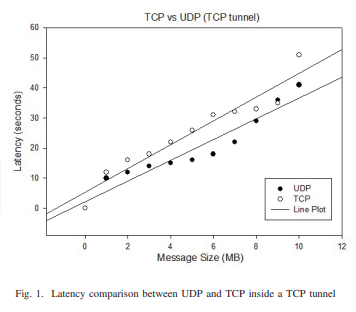
\includegraphics[width=\columnwidth]{Figures/TCPUDP-TCPTUN.png}
        \caption{Latency of TCP/UDP through TCP Tunnel~\cite{coonjah_experimental_2015}}
        \label{fig:tcpudp-tcptun}
      \end{figure}

      \begin{figure}[h]
        \centering
        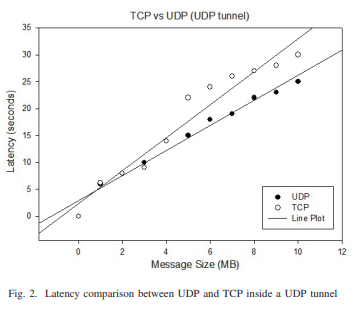
\includegraphics[width=\columnwidth]{Figures/TCPUDP-UDPTUN.png}
        \caption{Latency of TCP/UDP through UDP Tunnel~\cite{coonjah_experimental_2015}}
        \label{fig:tcpudp-udptun}
      \end{figure}


    \section{Network Models}
    \label{sec:networkModel}
      OSI, TCP/Internet Protocol (TCP/IP) and Information-Centric Networks (ICN) are three network model standards that offer different purposes for how the network handles the transmission of network packets. The OSI network model provides a layer abstraction that works in many network situations, making it a popular OSI model. OSI model contains seven layers, which are:-
      \begin{itemize}
        \centering
        \item[] \textbf{Layer 1:} Physical
        \item[] \textbf{Layer 2:} Data Link
        \item[] \textbf{Layer 3:} Network
        \item[] \textbf{Layer 4:} Transport
        \item[] \textbf{Layer 5:} Session
        \item[] \textbf{Layer 6:} Presentation
        \item[] \textbf{Layer 7:} Application
      \end{itemize}

      The structure of the TCP/IP model is as follows:-
      \begin{itemize}
        \centering
        \item[] \textbf{Layer 1:} Network Access
        \item[] \textbf{Layer 2:} Internet Protocol
        \item[] \textbf{Layer 3:} Transport
        \item[] \textbf{Layer 4:} Application
      \end{itemize}
    
      ICN uses three layers containing the following:-
      \begin{itemize}
        \centering
        \item[] \textbf{Layer 1:} ICN Application
        \item[] \textbf{Layer 2:} ICN Forwarding
        \item[] \textbf{Layer 3:} Link
      \end{itemize}

    \section{Network Syncronisation}

    \section{Implementation}

    \section{Conclusion}
    
    \section{Terminology}
      \begin{itemize}
        \item \textbf{TCP:} Transmission Control Protocol.
        \item \textbf{UDP:} User Datagram Protocol.
        \item \textbf{MTU:} Maximum Transmission Unit.
        \item \textbf{OSI:} Open Systems Interconnection.
        \item \textbf{IoT:} Internet of Things.
        \item \textbf{MB:} Megabytes.
        \item \textbf{IP:} Internet Protocol.
        \item \textbf{ICN:} Information-Centric Networks.
      \end{itemize}

  %\nocite{*}
	\renewcommand\refname{\section{Reference List}}
	\small{\bibliographystyle{IEEEtran}
    \bibliography{ref}}
\end{document}